\section{KFAC: initial approximation $\tilde{F}$}
\frame{\tableofcontents[currentsection, hideothersubsections]}

\begin{frame}
\frametitle{KFAC: initial approximation $\tilde{F}$}

\begin{figure}
    \centering
    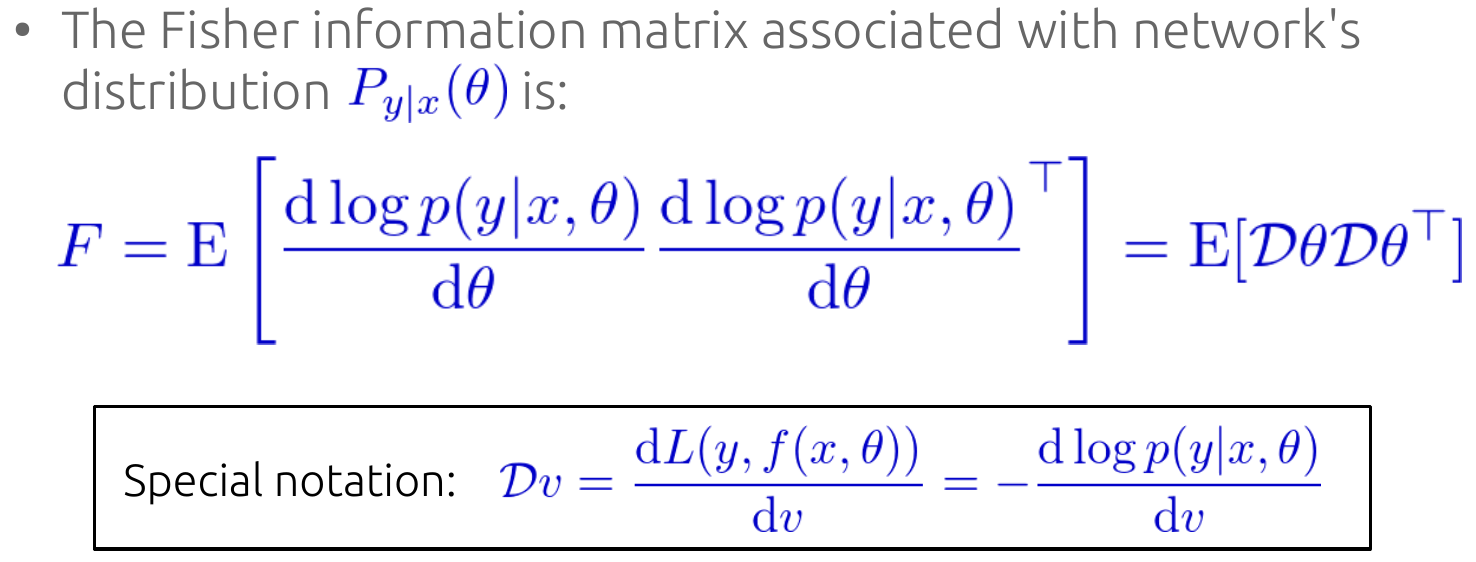
\includegraphics[scale=0.175]{fisher}
\end{figure}

\begin{figure}
    \centering
    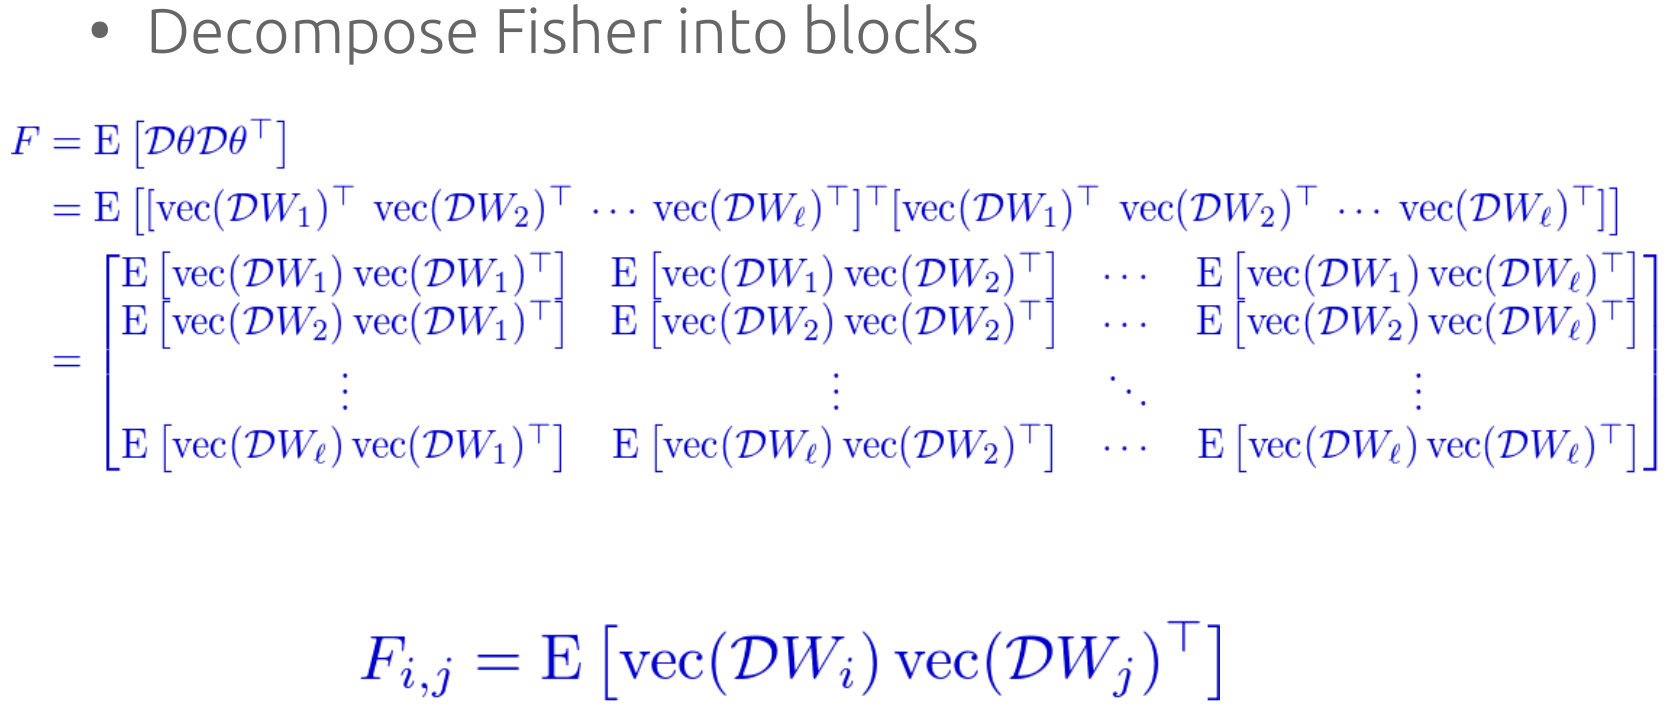
\includegraphics[scale=0.225]{kfac_01}
\end{figure}

\end{frame}

\begin{frame}
\frametitle{KFAC: initial approximation $\tilde{F}$}

\begin{figure}
    \centering
    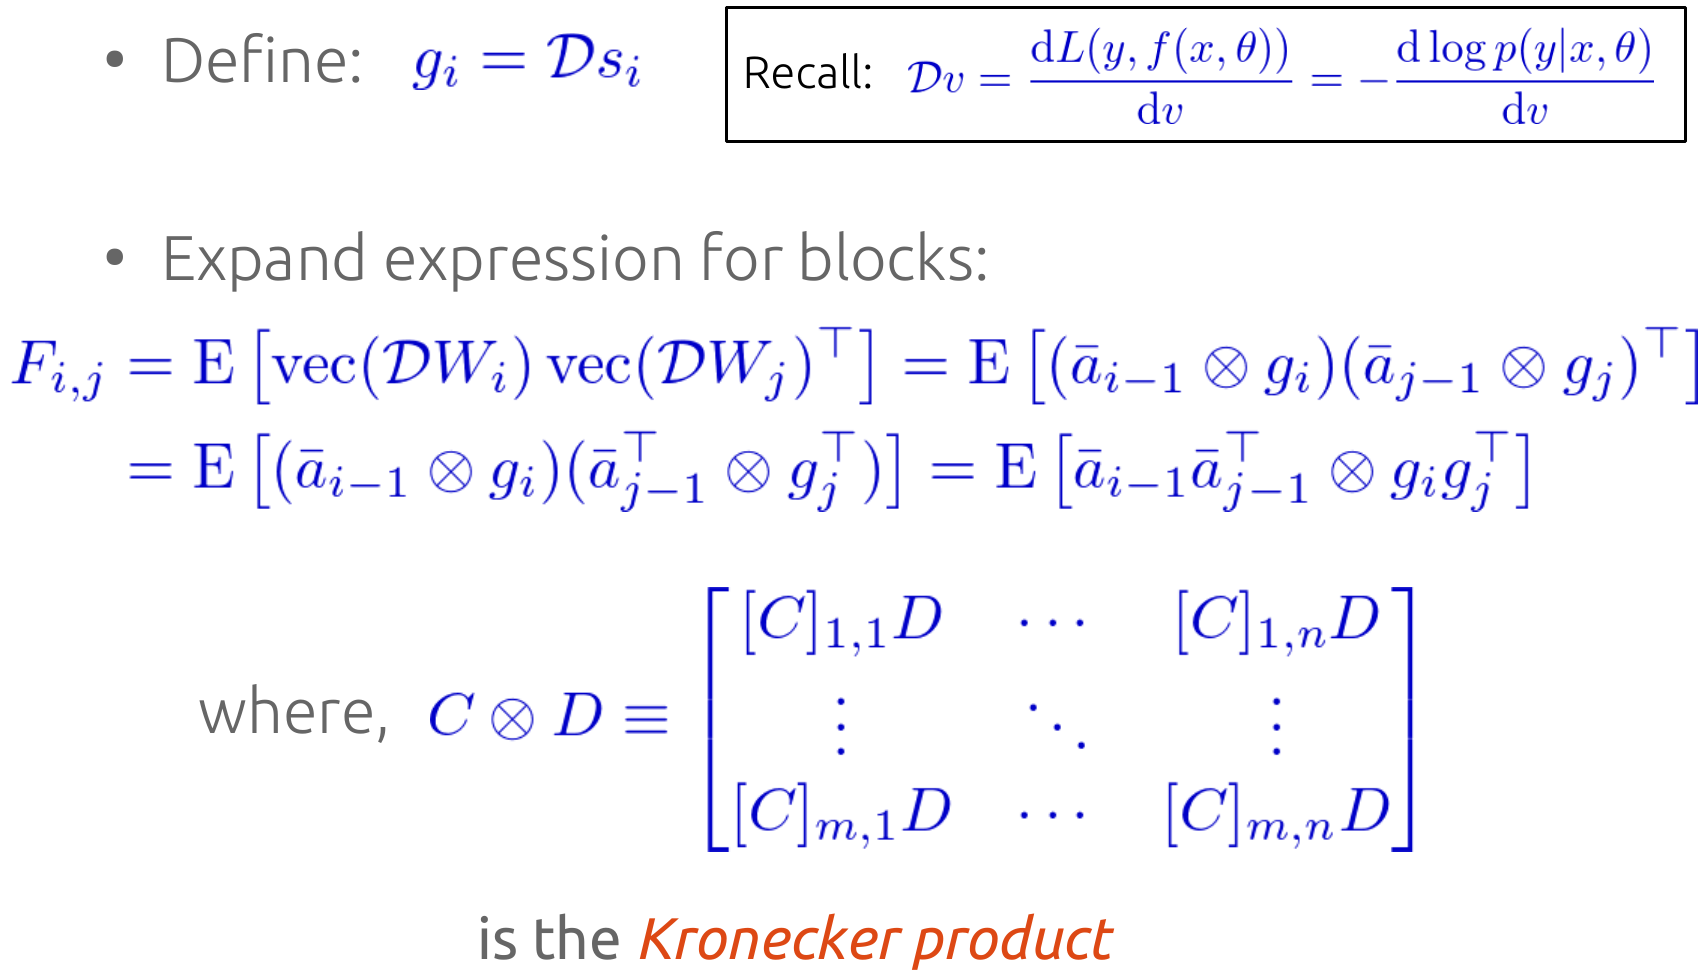
\includegraphics[scale=0.25]{kfac_02}
\end{figure}

\end{frame}

\begin{frame}
\frametitle{KFAC: initial approximation $\tilde{F}$}

\begin{figure}
    \centering
    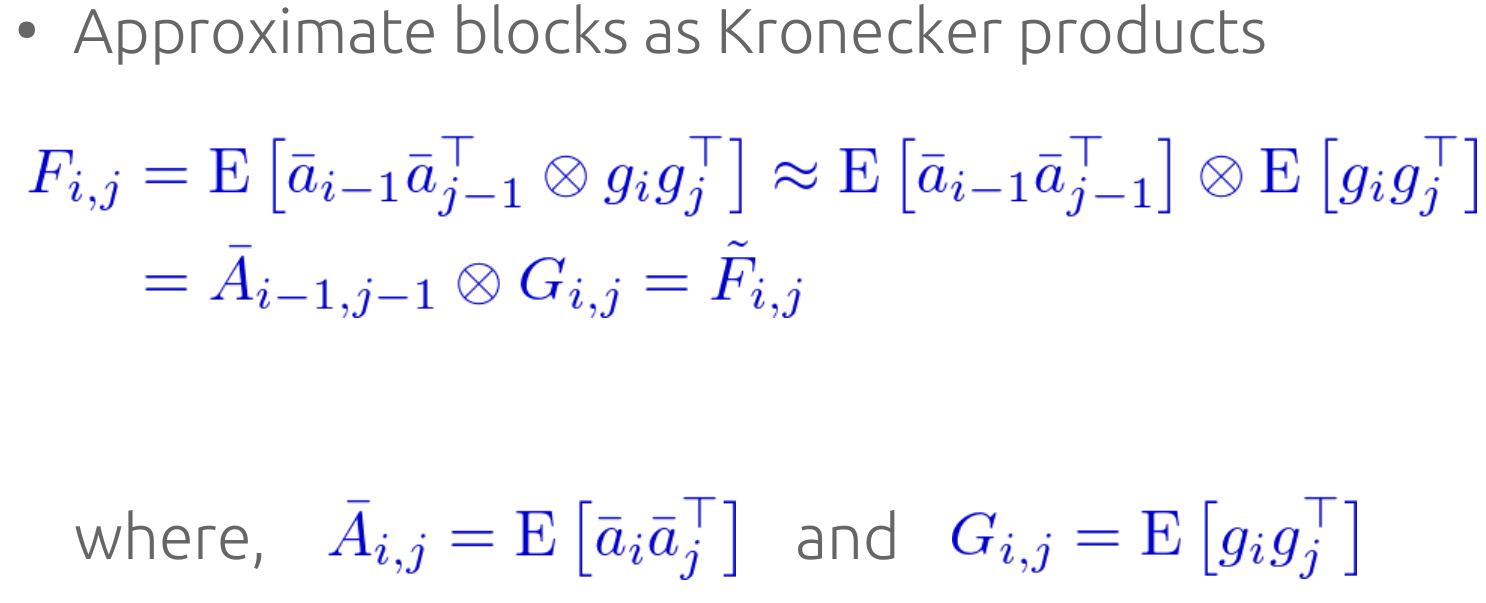
\includegraphics[scale=0.215]{kfac_03}
\end{figure}

\begin{figure}
    \centering
    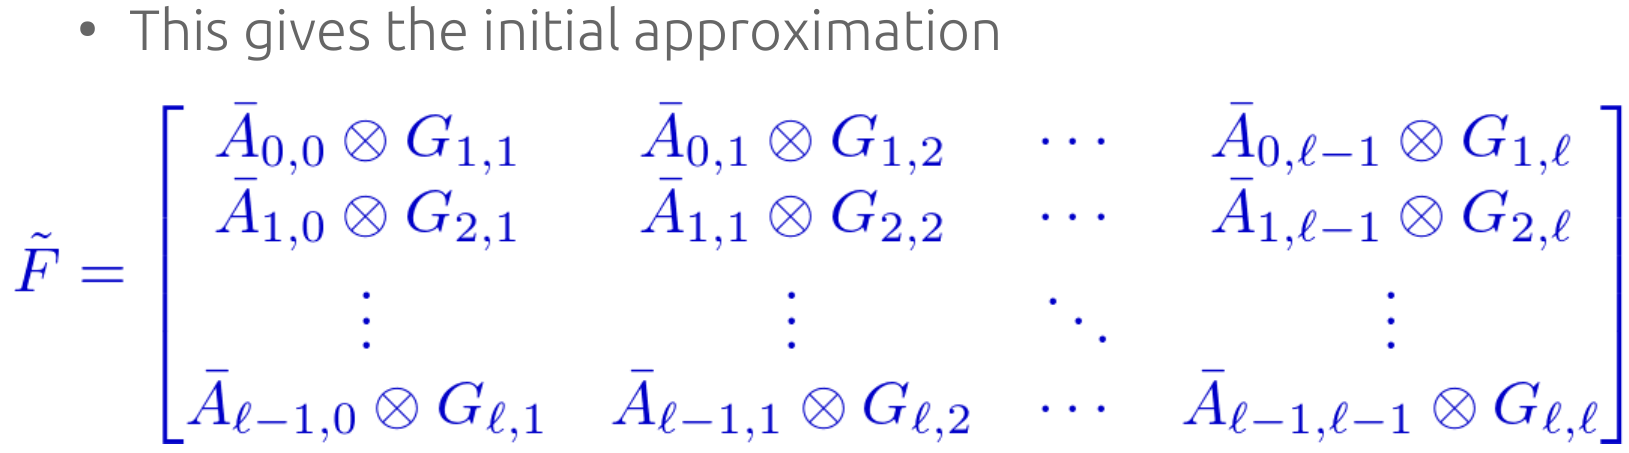
\includegraphics[scale=0.2]{kfac_04}
\end{figure}

Indeed a major approximation because\\
the expectation of a Kronecker product is, in general, NOT
equal to the Kronecker product of expectations

\end{frame}

\begin{frame}
\frametitle{KFAC: initial approximation $\tilde{F}$}
Comparing the exact $F$ vs its approximate $\tilde{F}$
\begin{figure}
    \centering
    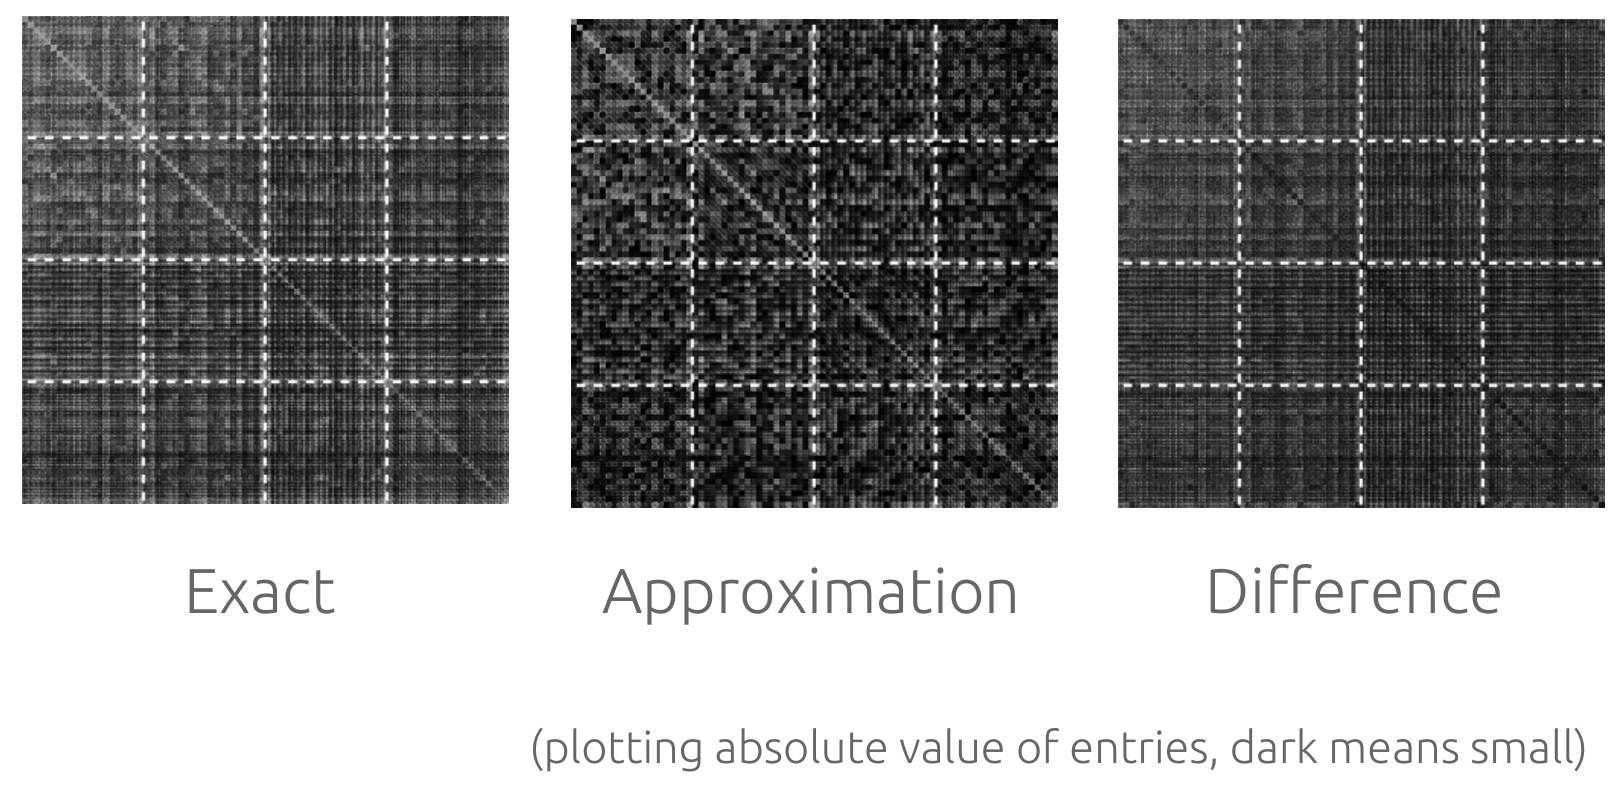
\includegraphics[scale=0.25]{kfac_05}
\end{figure}

\end{frame}


